\documentclass[12pt,a4paper]{report}
\usepackage{graphicx}
\usepackage{amsmath}
\usepackage{fancyhdr}
\usepackage{cite}
\usepackage{framed}
\usepackage{a4wide}
\usepackage{float}
\usepackage{blindtext}
\usepackage{multicol}
%The below Section make chapter and its name to center of the page
\usepackage{blindtext}
\usepackage{xpatch}
\usepackage{mathptmx}
\usepackage{geometry}
\usepackage{float}
\usepackage{caption}
\usepackage{subcaption}
\usepackage{babel,blindtext}
\usepackage{color}   %May be necessary if you want to color links
\usepackage{hyperref}

\hypersetup{
    colorlinks=true,
    linktoc=all,
    linkcolor=black,
    urlcolor  = black,
}

 \geometry{
 right=25mm,
 left=35mm,
 top=25mm,
 bottom=25mm,
 }
% \usepackage{fontspec}
\usepackage{tocloft}
\makeatletter
\renewcommand{\cftdot}{}
\renewcommand{\cftchappresnum}{CHAPTER }
\renewcommand{\cftchapaftersnum}{:}
\renewcommand{\cftchapnumwidth}{6.5em}
\renewcommand\cftfigindent{0pt}
\renewcommand\cftfigpresnum{Figure\ }
\renewcommand\cftfigaftersnum{ : }
\renewcommand{\cftfignumwidth}{5.5em}
\renewcommand{\cfttabpresnum}{Table\ }
\renewcommand\cfttabaftersnum{ : }
\renewcommand{\cfttabnumwidth}{5em}
\makeatother


% \setmainfont{Times New Roman}
\makeatletter
\xpatchcmd{\@makeschapterhead}{%
  \Huge \bfseries  #1\par\nobreak%
}{%
  \Huge \bfseries\centering #1\par\nobreak%
}{\typeout{Patched makeschapterhead}}{\typeout{patching of @makeschapterhead failed}}


\xpatchcmd{\@makechapterhead}{%
  \huge\bfseries \@chapapp\space \thechapter
}{%
  \huge\bfseries\centering \@chapapp\space \thechapter
}{\typeout{Patched @makechapterhead}}{\typeout{Patching of @makechapterhead failed}}

\makeatother

\linespread{1.5}

\begin{document}

\begin{center}
{\Huge \textbf{Texture Synthesis}}\\
\vspace{0.5cm}

\vspace{1 cm}
{\large {Submitted by:}} \\

% \begin{multicols}{3}
% \vspace{1cm}
{\Large \textbf{Aayush Goyal}}
% \vspace{0.2cm}
{\Large \textbf{(2019CS10452)}}
% \vspace{0.2cm}

\vspace{0.2cm}
% \end{multicols}
\vspace{1 cm}
{\large {Under the supervision of}}\\

{\Large \textbf{Prof. Prem Kalra}}\\

\end{center}

\vspace{6pt}
\begin{center}
\begin{figure}[H]
    \centering
    
\includegraphics[scale=0.1]{pics/iitd.png}
    \label{fig:DTU logo}
\end{figure}
{\Large \textbf{COD 310, Mini Project}}\\

{\large \textbf{Indian Institute of Technology, Delhi}}\\

\end{center}

\thispagestyle{empty}

\newpage



\newpage

\begin{center}
  {\Huge \textbf{Abstract}}
  \addcontentsline{toc}{chapter}{Abstract}
\end{center}
\vspace{0.8cm}
Texture Synthesis is a topic of study in computer graphics and is used in a variety of fields such as fashion, digital image editing, and medicine. We want to expand its application in the medical industry. Our main goal is to generate larger instances that perceptually resemble the smaller input texture exemplar given some small texture of parts of our body. The main idea is to use a patch-based method for generating visual appearance i.e. new image is synthesised by intelligently stitching together small patches of an existing image.

\newpage

\tableofcontents

\newpage

\pagenumbering{arabic}    
\chapter{ Introduction}


\section{What is Texture Synthesis?}
It is a method for producing arbitrarily large textures from small real-world samples. The idea is that we take an input image of a texture and then look for other images that look similar to that texture. So the assumption here is that somewhere out there, in the real world there exists larger texture and the input image is just a small sample and we want to get just some more samples of that texture. One of the assumptions here is that the input image is large enough to capture the essence of this texture.
\\\\
The main challenge for texture synthesis is that there are many different textures, such as some that are purely \textbf{repeated} (look like somewhat regular patterns), some that are \textbf{stochastic} (texture images of stochastic textures look like noise), and most that fall somewhere in between the \textbf{mix} of repeated and stochastic.
\vspace*{0.8cm}


\begin{figure}[H]
  \centering
\minipage{0.32\textwidth}
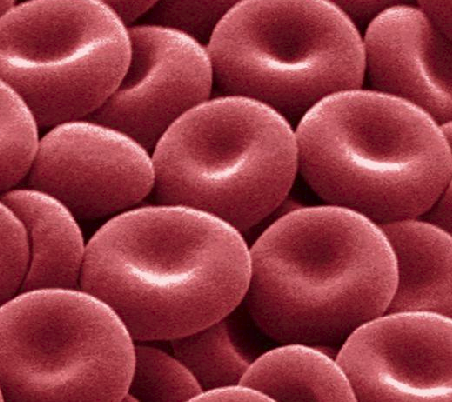
\includegraphics[scale=0.3]{pics/rbc_sample.png}
  \caption*{(a) Repeated (RBCs)}
\endminipage
\hspace*{0.5cm}
\minipage{0.32\textwidth}
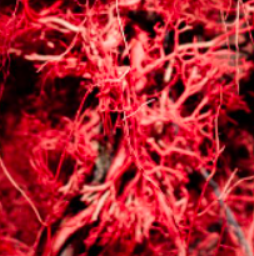
\includegraphics[scale=0.47]{pics/blood_vessels.png}
  \caption*{(b) Stochastic (BVs)}
\endminipage
\minipage{0.32\textwidth}%
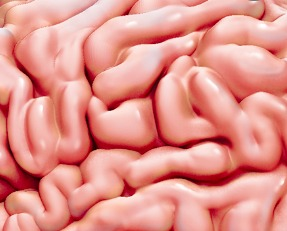
\includegraphics[scale=0.52]{pics/brain.jpeg} 
  \caption*{(c) Both (Brain)}
\endminipage
\end{figure}


\section{Problem Formulation}
We want to expand its application in the medical industry. When we provide the algorithm a small sample of the texture of a region of our body, the primary objective is to produce larger examples that visually resemble the smaller input texture exemplar. The user will provide input in the form of an image, and they will be able to select the size of the texture that they wish to generate. The final product will be a newly generated texture that looks very much like the image that was input. The primary concept behind this is the utilisation of a patch-based method for the generation of visual appearance. This means that a new image is created by cleverly piecing together small patches of an already existing image.



\chapter{Proposed Method}

\section{About Patch-Based Method}
We'll look at a patch-based technique also known as \textbf{Image Quilting}. First, we will define the synthesis unit \textbf{Bi}, which is a square block whose size is defined by the user. We've assigned set \textbf{S} to all of these square blocks, which are overlapping blocks from input image.
\\\\
The most basic and naive approach is \textbf{Random Block Placement}, in which we randomly select patches from the input texture and place them on a larger target image. This can be accomplished by looping from left to right, top to bottom (rendering order), and placing randomly sampled blocks from \textbf{S} next to each other.

\begin{figure}[H]

\minipage{0.25\textwidth}
\centering
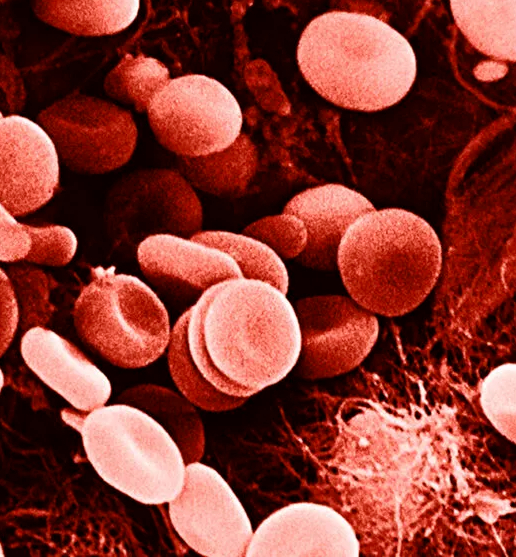
\includegraphics[scale=0.19]{pics/rbc_input.jpg}
\caption*{(a) Input image}
\endminipage\hspace*{0.5cm}
\minipage{0.25\textwidth}
\centering
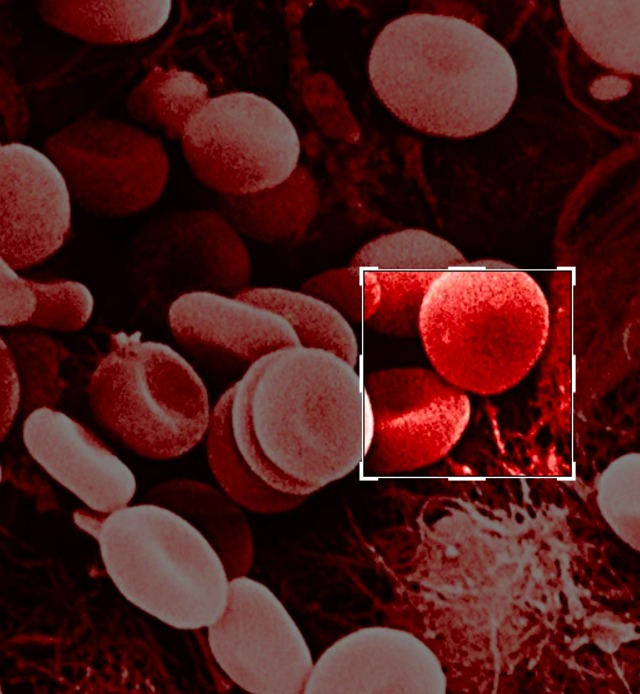
\includegraphics[scale=0.15]{pics/rbc_bi.jpg}
\caption*{(b) Choosing a Patch}
\endminipage
\minipage{0.5\textwidth}
\centering
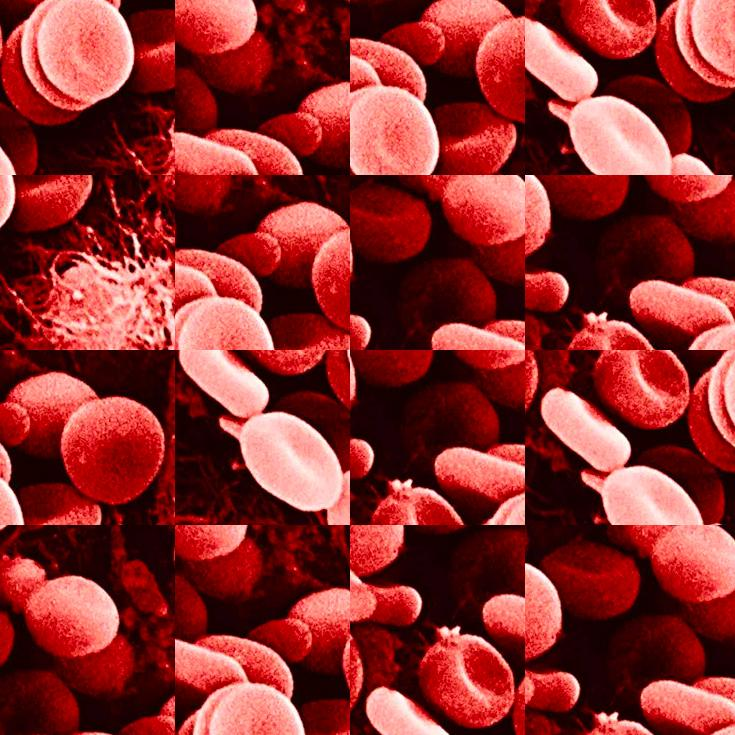
\includegraphics[scale=0.23]{pics/rbc_random.jpg}
  \caption*{(c) Output by Random Placement}\label{fig:awesome_image2}
\endminipage
\caption*{We can see that the blocks do not match, and the output image is not satisfying.}

\end{figure}

\section{Using Neighboring Block constrained by Overlap}
As we can see in the image output created by selecting random patches from the input texture, the blocks do not match. The output image has visible edges, as we can see. So we must overcome this. We'll accomplish this by using \textbf{Neighboring Block constrained by Overlap}, which will cause some overlap in the placement of blocks on the new image. The top left patch is chosen at random, and the next patch from \textbf{S} is chosen to minimise the overlap error \textbf{L2 norm}. The new block is partially overlaid on the previous block, starting from the centre.

% TODO: If I do the parallelization, mention it here in the bold

\begin{figure}[H]

  \minipage{0.5\textwidth}
  \centering
  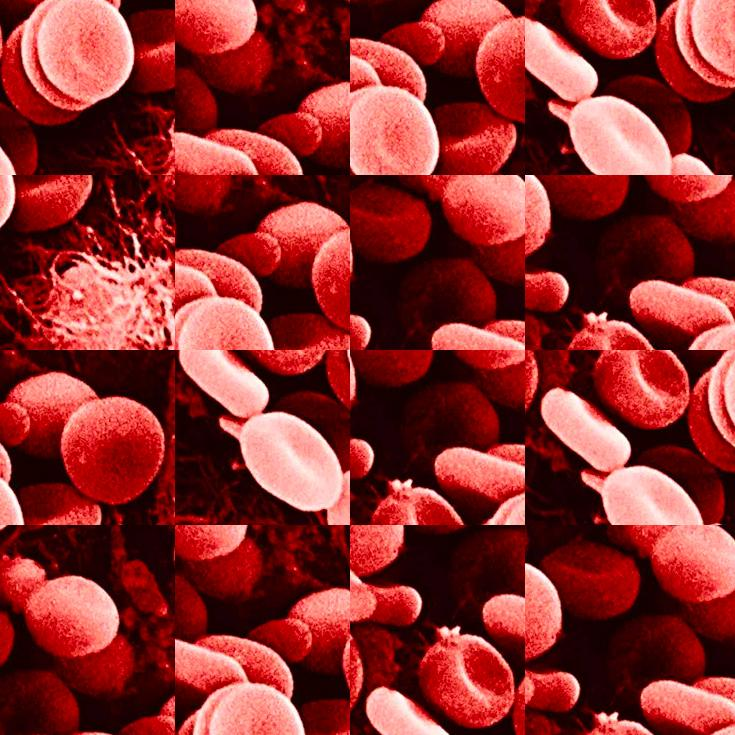
\includegraphics[scale=0.23]{pics/rbc_random.jpg}
  \caption*{(a) Ouput image formed by placing blocks Randomly}
  \endminipage\hspace*{0.5cm}
  \minipage{0.5\textwidth}
  \centering
  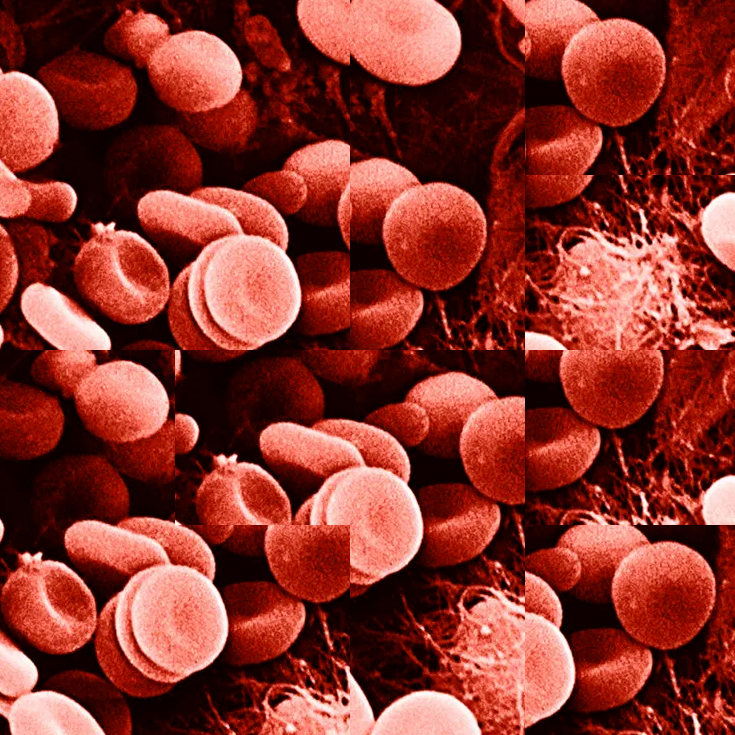
\includegraphics[scale=0.23]{pics/rbc_best.png}
    \caption*{(b) Ouput formed by placing blocks based on Neighboring Block constrained by Overlap}
  \endminipage
  \newline 
  \caption*{The above image (b) shows an improvement in the target image's structure; the edges have been smoothed compared to (a), but the edges between the blocks are visible.}
  
\end{figure}
\newpage 
\section{Minimum Error Boundary Cut method}
Instead of a straight line between the two patches, we can use the Minimum Error Boundary Cut method to remove these visible edges. Before inserting a selected block into the target image, we inspect the overlap region between it and the other blocks for errors. We find the cheapest path through the error surface and declare it the boundary of the new block.
\newline 
\begin{figure}[H]

  \minipage{0.5\textwidth}
  \centering
  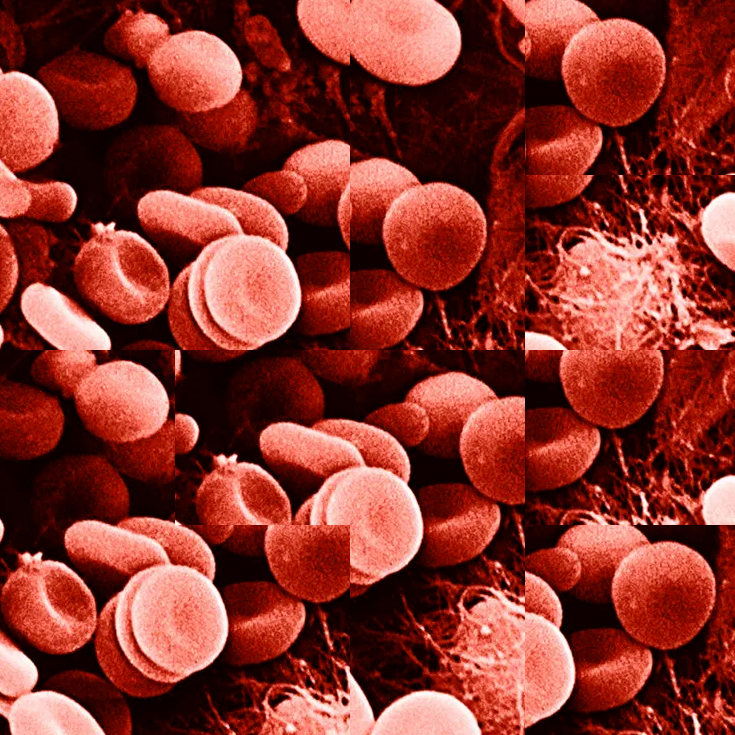
\includegraphics[scale=0.23]{pics/rbc_best.png}
    \caption*{(a) Ouput formed by placing blocks based on neighboring block constrained by overlap}
  \endminipage\hspace*{0.5cm}
  \minipage{0.5\textwidth}
  \centering
  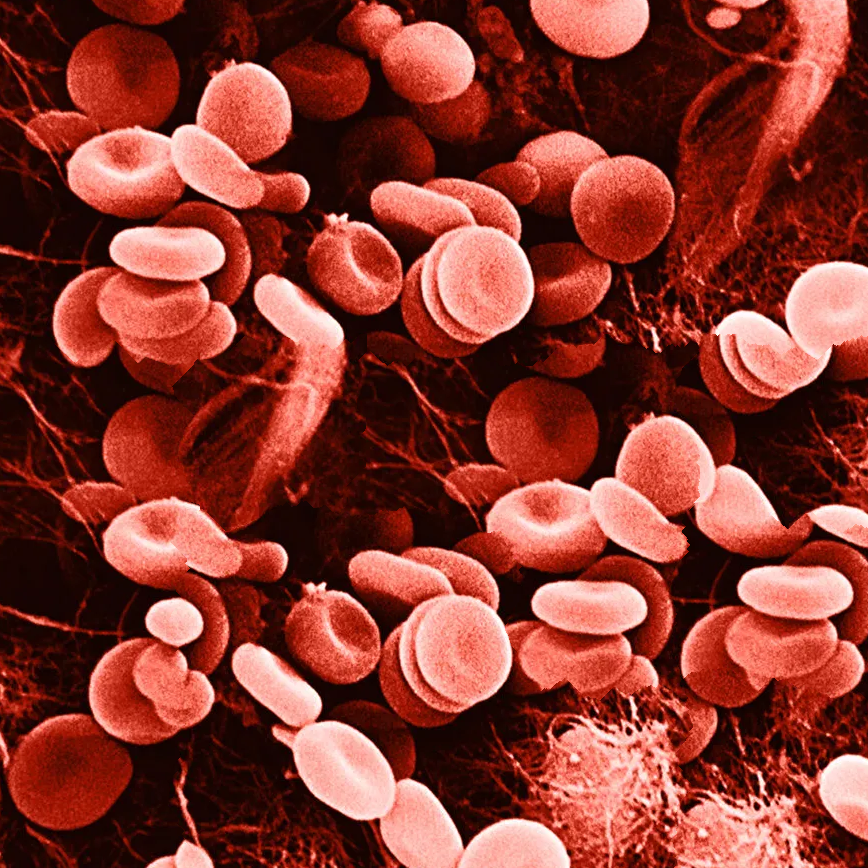
\includegraphics[scale=0.2]{pics/rbc_cut.png}
    \caption*{(b) Ouput formed by placing blocks with minimum error boundary cut}
  \endminipage
  \newline 
  \caption*{Above image (b) shows that the generated output is satisfying and edges are also smooth.}
  
\end{figure}



\chapter{Results and Discussion}


\section{Results}
We have introduced image quilting, a method of syn-
thesizing a new image by stitching together small patches of existing images. Despite its simplicity, this method works remarkably well when applied to texture synthesis, producing highly stable results. For wide variety of input textures, the result of texture synthesis can be seen below.
\newline
\begin{figure}[H]
  \centering
  \minipage{0.4\textwidth}
  \centering
  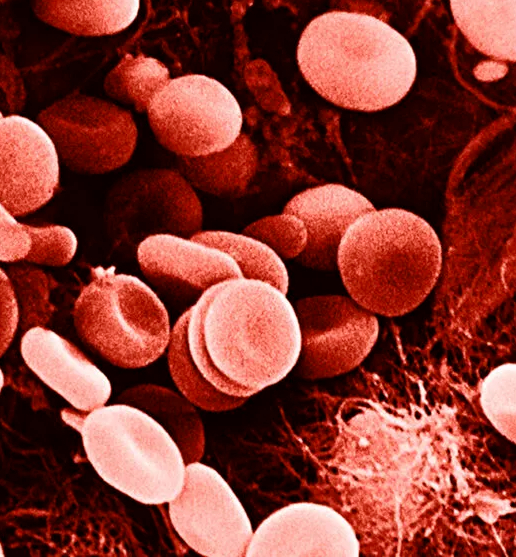
\includegraphics[scale=0.22]{pics/rbc_input.jpg}
  \caption*{(a) Input image}
  \endminipage
  \minipage{0.6\textwidth}
  \centering
  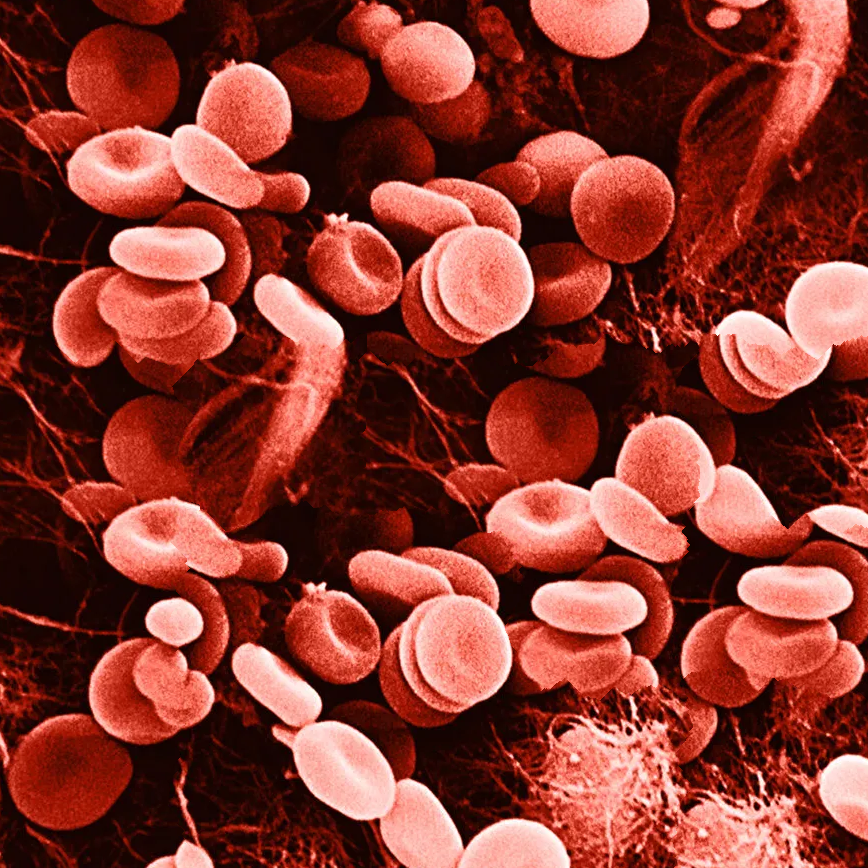
\includegraphics[scale=0.25]{pics/rbc_cut.png}
    \caption*{(b) Output Image}
  \endminipage
  \caption{Input is an image of human Red Blood Cells. The size of input is 516 x 557 pixels. A block size of 200 will be able to cover the components like individual cell and nerves. The size of output image is 868 x 868 pixels.}
  
\end{figure}


\begin{figure}[H]
  \centering
  \minipage{0.4\textwidth}
  \centering
  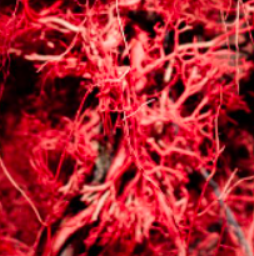
\includegraphics[scale=0.45]{pics/blood_vessels.png}
  \caption*{(a) Input image}
  \endminipage
  \minipage{0.6\textwidth}
  \centering
  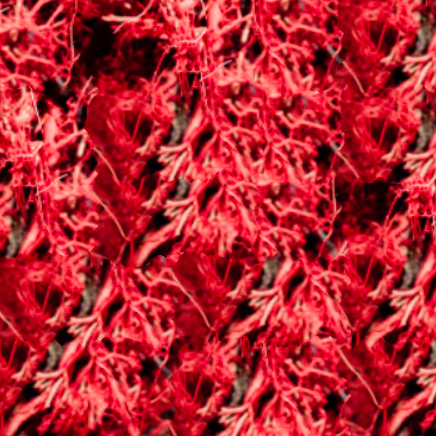
\includegraphics[scale=0.5]{pics/blood_vessels_100_5.png}
    \caption*{(b) Output Image}
  \endminipage
  \caption{Input is an image of human Blood vessels. Size of input is 254 x 256 pixels. Block size of 100 will be appropriate. The size of output image is 436 x 436 pixels.}
  
\end{figure}


\begin{figure}[H]
  \centering
  \minipage{0.4\textwidth}
  \centering
  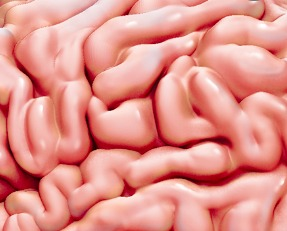
\includegraphics[scale=0.42]{pics/brain.jpeg}
  \caption*{(a) Input image}
  \endminipage\hspace*{0.2cm}
  \minipage{0.6\textwidth}
  \centering
  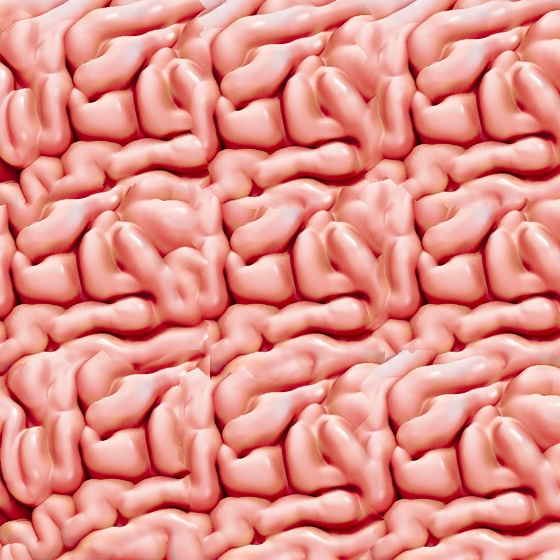
\includegraphics[scale=0.4]{pics/brain_210_3.png}
    \caption*{(b) Output Image}
  \endminipage
  \caption{Input is an image of human Brain. Size of input is 287 x 231 pixels. Block size of 210 will be appropriate, taking it less than that will produce noise in the output. The size of output image is 560 x 560 pixels.}
  
\end{figure}

\newpage 

\section{Discussion}
\begin{enumerate}
  \item The algorithm performs well on stochastic and very regular textures, but user-specified parameters such as block size, number of blocks, and input texture type all had a significant impact on the quality of the results. One of the big assumptions here is that the input image is large enough to capture the essence of this texture. Then we should cleverly choose the block size. The block size should be chosen in such a manner that it is able to capture the different components of the texture. Like in case we have an input image of Red blood cells, an appropriate block size would be something that covers one cell roughly. It should not be too small or large.
  \item The time taken to generate the output highly depends on the size of the input image and the block size (Bi) chosen by us. The larger the input size and the lesser the block size, more time is required to generate the output. Further it also increases proportionally with the number of blocks. The more the number of blocks, the bigger the image will be and the more time it will take to generate the output. Let's say the block size is $B$ pixels, number of blocks is $N$, and the overlap region is $V$ pixels. Then the size of the output is: $NB - (N-1)V$. Currently the value of overlap size is set to $\frac{1}{6}^{th}$ of the Block size.
\end{enumerate}


\chapter{Scope of Future Work}
% write something about the Future possibilities. let's say

% 1) About how we can speed up the process by running it in multiple threads. When we are going through the set of all possible patches, we can do that in parallel.

One of the major limitations of this algorithm, as discussed above, is that it requires the input image to be large enough to cover the essence of the larger texture that we want to generate. Also, the output image is created by stitching together patches from the input image itself. As a result, there is no possibility of new features being introduced into the larger output image. Deep learning-based methods can be used to overcome this. Not only that, they are effective in limiting the output to specific boundaries. Let's say we have a texture for some part of the brain and want to expand it to the entire sketch of the brain, then it is possible to do this using models trained using these algorithms. This research was published in the paper \cite[TextureGAN: Controlling Deep Image Synthesis with Texture Patches]{b2}. They have provided examples based on clothing and footwear. Essentially, they enter a small texture as the design for the shoe or cloth, followed by the sketch of the shoe or cloth. The model generates an output in which the texture has been expanded to cover the entire object. However, due to a lack of medical data, we do not currently have enough data to train the model for medical applications. If we can obtain the medical data, we can use this model to generate output for medical applications.

\begin{figure}[H]
  \centering
  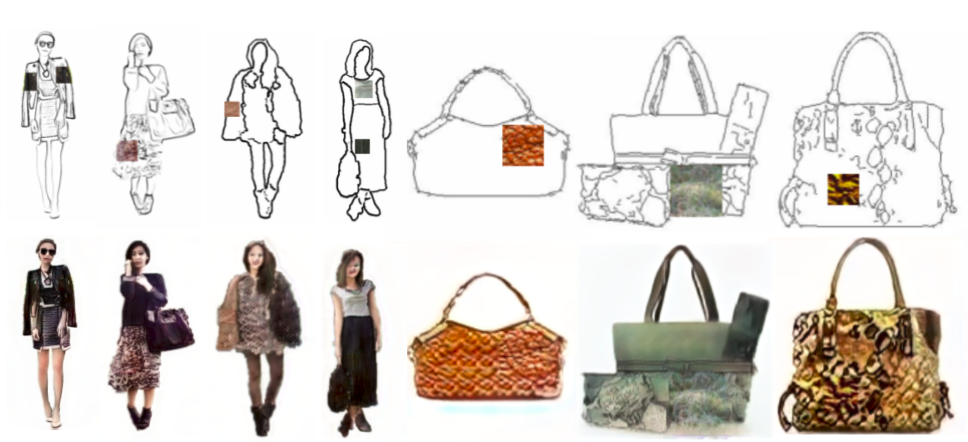
\includegraphics[scale = 0.33]{pics/examples.png}
\end{figure}

\addcontentsline{toc}{chapter}{References}

\begin{thebibliography}{99}
\bibitem{b1} \href{https://people.eecs.berkeley.edu/~efros/research/quilting/quilting.pdf}{Alexei A. Efros, William T. Freeman. Image Quilting for Texture Synthesis and Transfer. University of California, Berkeley. Mitsubishi Electric Research Laboratories.}
\bibitem{b2} \href{https://arxiv.org/pdf/1706.02823v3.pdf}{Wenqi Xian, Patsorn Sangkloy, Varun Agrawal, Amit Raj, Jingwan Lu, Chen Fang, Fisher Yu, James Hays. TextureGAN: Controlling Deep Image Synthesis with Texture Patches. Georgia Institute of Technology, Adobe Research, UC Berkeley.}
\bibitem{b3} \href{https://arxiv.org/pdf/1805.04487v1.pdf}{Yang Zhou, Zhen Zhu, Xiang Bai, Dani Lischinski, Dani Lischinski, Hui Huang. Non-Stationary Texture Synthesis by Adversarial Expansion}
\end{thebibliography}


\end{document}

